% This must be in the first 5 lines to tell arXiv to use pdfLaTeX, which is strongly recommended.
\pdfoutput=1
% In particular, the hyperref package requires pdfLaTeX in order to break URLs across lines.

\documentclass[11pt]{article}

% Remove the "review" option to generate the final version.
\usepackage[]{FinalReport/report}

% Standard package includes
\usepackage{times}
\usepackage{latexsym}
\usepackage[T1]{fontenc}
\usepackage[utf8]{inputenc}
\usepackage{microtype}
\usepackage{inconsolata}
\usepackage{natbib}
\usepackage{tikz}
\usepackage{tikzscale}
\usepackage{float}
\usepackage{pgfplots}
\usepackage{pgfplotstable}
\usepackage{amssymb}

\newcommand{\todo}[1]{[\textcolor{red}{\textit{TODO: }{#1}}]}

\title{15-618 Final Project: Sparse Attention in CUDA}

\author{Sarah Di \\
  Carnegie Mellon University\\
  \texttt{sarahdi@andrew.cmu.edu} \\\And
  Jinsol Park \\
  Carnegie Mellon University\\
  \texttt{jinsolp@andrew.cmu.edu} \\}

\begin{document}
\maketitle
\begin{abstract}
We implemented sparse attention on CPU and GPU platforms using C++ and CUDA respectively, and compared the performance of the two implementations using a variety of tiling methods.
\todo{Add in what our results , is X effective? which tiling method is the most effective? How much speedup did that method get?}


\todo{What machines they ran on}

\end{abstract}

\section{Background}
Transformers are powerful deep learning models that excel at tasks in various fields including natural language processing, computer vision, and audio processing \cite{lin2022survey}. 

The Transformer as described in \citet{vaswani2017attention} is comprised of encoder and decoder stacks. \todo{should there be a picture of the transformer model?} An encoder block consists of a multi-head self-attention module followed by a position-wise fully-connected feed-forward network. The encoder layer also contain additional Add \& Normalization steps. Decoder blocks are similar but contain additional cross-attention layers inserted between the multi-head attention and feed-forward network layers.
\subsection{Attention}
The attention layer plays a vital role in the Transformer, as it allows the model to capture long-range relationships via similarity scores for all item pairs in a sequence \cite{khan2022transformers}. 

\todo{explain that it's composed of matmuls + softmax, explain Query Key structure, }
\todo{key data structures? key operations on these data structures? algo's inputs and outputs? }

However, the complexity of self-attention is $O(T^2D)$, where $T$ is the sequence length and $D$ is the representation dimension. To validate this, we captured the computation time of layers within BERT\footnote{We used Hugging Face's BERT model \url{https://huggingface.co/docs/transformers/model_doc/bert}}, an encoder-only language model developed in 2018 \cite{devlin2018bert}. For \autoref{fig:berttiming}, notice that as the sequence length increases, the computational time of the Self-Attention layer, as shown in green, scales quadratically. The time, measured in seconds, is also shown in \autoref{fig:bertTimes}.
\begin{figure}[H]
\pgfplotstableread{
    Label SelfAttention SelfOutput FeedForward Output topper
    128 0.079665  0.019992 0.084192 0.073205 0.001
    256 0.300243  0.040303 0.153612 0.147656 0.001
    512 0.545014 0.078534 0.322093 0.282523 0.001
    1024 3.854414 0.193473 0.686376 0.707752 0.001
    %2048 13.631169 0.332429 1.277496 1.172507 0.001
        }\testdata
    \centering
    \includegraphics[width=\linewidth]{bertTimingPlot.tikz}
    \caption{Computational Times for BERT layers vs Sequence Length}
    \label{fig:berttiming}
\end{figure}
\begin{table*}[h!]
\centering
 \begin{tabular}{||c | c c c c||} 
 \hline
 Sequence Length & Attention & Add \& Norm & FeedForward & Add \& Norm \\ [0.5ex] 
 \hline\hline
 128 & 0.079665 & 0.019992 & 0.084192 & 0.073205 \\
 256 & 0.300243 & 0.040303 & 0.153612 & 0.147656 \\
 512 & 0.545014 & 0.078534 & 0.322093 & 0.282523 \\
 1024 & 3.854414 & 0.193473 & 0.686376 & 0.707752 \\
 2048 & 13.631169 & 0.332429 & 1.277496 & 1.172507 \\ [1ex] 
 \hline
 \end{tabular}
  \caption{Computational Times (in seconds) for BERT layers vs
Sequence Length}
  \label{fig:bertTimes}
\end{table*}
Since both the memory and computational complexity scale quadratically with sequence length, attention becomes a performance bottleneck on longer sequences. One way to reduce computational costs is to introduce a sparsity bias into the attention module \cite{child2019generating}.
\subsection{Sparse Attention}
Sparse attention differs from normal attention in that it computes only a limited number of similarity scores for a sequence. By factorizing the attention matrix to only compute certain parts, sparse attention reduces the total computation complexity to $O(T\sqrt{T})$. \todo{Big Bird disc. more stuff about how it approximates full attention} Different factorization methods \cite{zaheer2020big, beltagy2020longformer} of the attention matrix lead to different sparse attention modes. Some such sparse attention modes are:
\begin{figure*}[h]
  \centering
  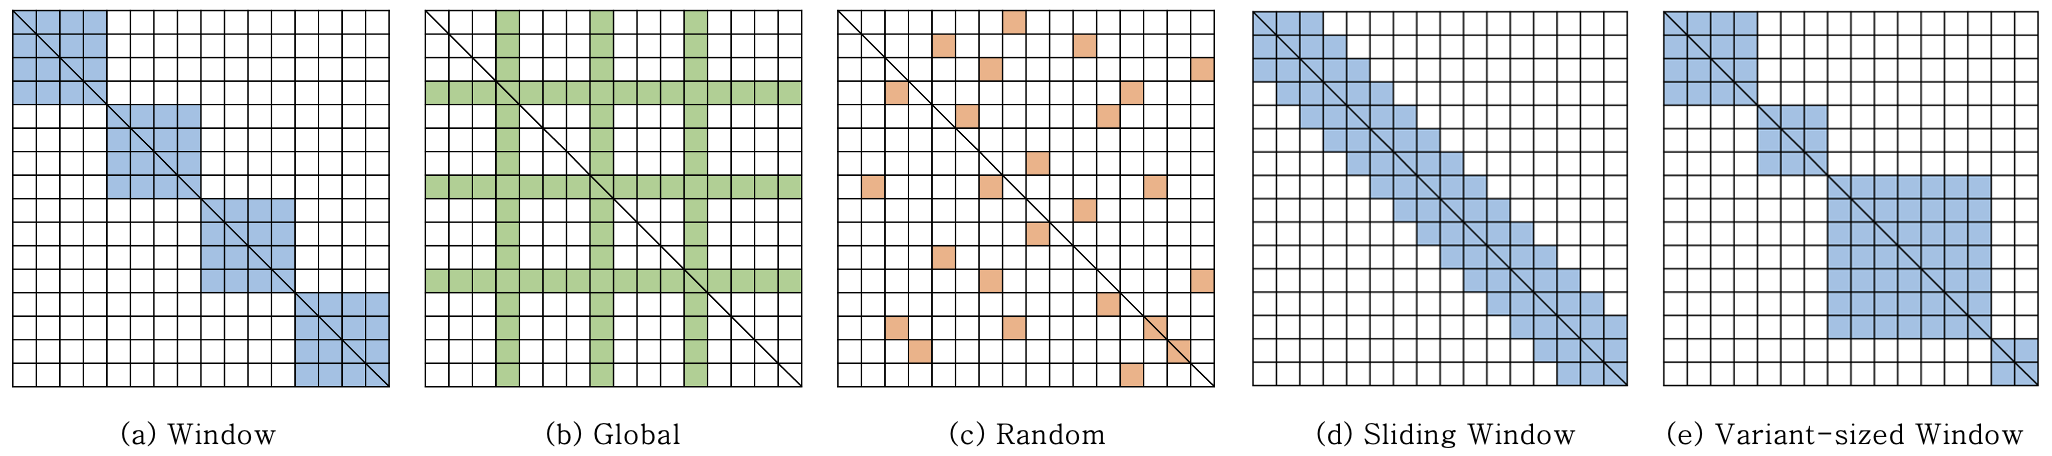
\includegraphics[width=\linewidth]{figures/building_block.png}
  \caption{Different factorization methods of sparse attention.  Each connectivity matrix shows whether an $i^{th}$ token (row) of a sequence refers to a $j^{th}$ token (column) to compute an attention score. These can be combined to be a single sparse attention method.}
 \label{fig:bulding_block}
\end{figure*}
\begin{itemize}
    \item \textbf{Window attention}: \autoref{fig:bulding_block} (a)
    \item \textbf{Global attention}: \autoref{fig:bulding_block} (b)
    \item \textbf{Random attention}: \autoref{fig:bulding_block} (c)
\end{itemize}
\todo{mention why sparse attention could benefit for parallelization/exploiting shared memory}
\todo{Break down the workload. Where are the dependencies in the program? How much parallelism is there? Is it data-parallel? Where is the locality? Is it amenable to SIMD execution?}
\section{Approach}

Tell us how your implementation works. Again, it might be very useful to include a figure here illustrating components of the system and/or their mapping to parallel hardware.
\subsection{Technology}
We implemented our own Attention module in C++ 
\todo{Describe the technologies used. What language/APIs? What machines did you target?}

\todo{Describe how you mapped the problem to your target parallel machine(s). IMPORTANT: How do the data structures and operations you described in part 2 map to machine concepts like cores and threads. (or warps, thread blocks, gangs, etc.)}
\subsection{Naive Attention Implementation}
\todo{Did you change the original serial algorithm to enable better mapping to a parallel machine?}

\todo{If your project involved many iterations of optimization, please describe this process as well. What did you try that did not work? How did you arrive at your solution?}

\subsection{Window Attention}
\subsection{Global Attention}
\subsection{Random Attention}
\subsection{Shared Memory Cache Blocking}
\section{Results}
How successful were you at achieving your goals?
\todo{define how you measured performance, wall-clock time? Speedup? Application specific rate? (e.g., moves per second, images/sec)}
\todo{describe experimental setup. What were the size of the inputs? How were requests generated?}

\todo{add graphs of speedup or execute time. Precisely define configurations being compared. What is the baseline? single-threaded CPU code? parallel impl for a single CPU?}
\subsection{Problem Size}
\todo{do different workloads exhibit different execution behavior? Is it important to report results for different problem sizes for your project?}

\subsection{Limitations}
\todo{What limited your speedup? Lack of parallelism? (dependencies), Communication or synchronization overhead? Data transfer (memory-bound or bus transfer bound). Poor SIMD utilization due to divergence? provide data and measurements to support your conclusions. (or if speculating state this explicitly)}

\subsection{Deeper Analysis}
\todo{Can you break execution time of your algorithm into a number of distinct components. What percentage of time is spent in each region? Where is there room to improve?}

\todo{Was your choice of machine target sound? (If you chose a GPU, would a CPU have been a better choice? Or vice versa.)}

\section{List of work by each student, Distribution of Total Credit}
\todo{Please list the work performed by each partner. Given that you worked in a group, how should the total credit for the project be distributed amongst the participants?}
\begin{table}[h!]
\centering
 \begin{tabular}{||c | c c||} 
 \hline
 Task & Jinsol & Sarah \\ [0.5ex] 
 \hline\hline
 Literature Review & \checkmark& \checkmark\\
 Someother thing & &\\
 Someother thing & &\\
 Someother thing & &\\
 Someother thing & &\\
 Milestone Report & \checkmark & \checkmark\\
 Correctness Checks & \checkmark & \checkmark\\
 Profiling and Analysis & \checkmark & \checkmark\\
 Final Report & \checkmark & \checkmark\\
 Poster & \checkmark & \checkmark\\[1ex] 
 \hline
 \end{tabular}
  \caption{Work Distribution}
  \label{fig:bertTimes}
\end{table}
% Entries for the entire Anthology, followed by custom entries
\bibliographystyle{plainnat}
\bibliography{FinalReport/custom}

\appendix

\section{Appendix}
\label{sec:appendix}

This is a section in the appendix.

\end{document}